\documentclass[11pt,a4paper]{report}
\usepackage[T1]{fontenc}
\usepackage[latin1]{inputenc}
\usepackage{lmodern}
\usepackage{xcolor}
\usepackage{mathptmx}
\usepackage{graphicx}
\usepackage{hyperref}
\usepackage{listings}
\usepackage{adjustbox}

\begin{document}




  \begin{titlepage}
    \centering
    \fontsize{22}{32}\selectfont {Virtual Machine Software Testing}\\[0.5\baselineskip]
     \fontsize{17}{27}\selectfont {Internship Report}\\[1.5\baselineskip]
    
    
    
    \fontsize{11}{20}\selectfont \it {Submitted to:} \\[0.2\baselineskip]    
    \fontsize{12}{21}\selectfont {Student Internship Bureau }\\[0.3\baselineskip]    
    \fontsize{12}{21}\selectfont  {University of York, UK }\\[0.3\baselineskip]    



\begin{figure}[h]
\centering
\parbox{5cm}{

\includegraphics[width=3.5cm]{uniLogo.png}
%\caption{First.}
\label{fig:2figsA}}
\qquad
\begin{minipage}{5cm}

\includegraphics[width=3.5cm]{rapitaLogo.png}
%\caption{Second.}
\label{fig:2figsB}
\end{minipage}
\end{figure}

\bigskip
\bigskip

 \fontsize{11}{20}\selectfont \it {Submitted by:}\\[0.2\baselineskip]    
     \fontsize{12}{21}\selectfont {Mian Asbat Ahmad, PhD. Final Year }\\[0.1\baselineskip]
      \fontsize{12}{21}\selectfont {Department of Computer Science}\\[0.1\baselineskip]    
     \fontsize{12}{21}\selectfont  {University of York, UK }\\[1\baselineskip]    


\bigskip
     
     \fontsize{12}{22}\selectfont \it {Supervisors: Jennifer Mowat and Ian Broster} \\[1\baselineskip]    
     \fontsize{12}{22}\selectfont \it {Reviewer: Dr. Manuel Oriol} \\[0.5\baselineskip]    
   %   {\fontsize{13}{23}\selectfont Ian Broster, Rapita Sytstems Ltd. (host)}\\[2\baselineskip]
    
    \bigskip \bigskip
     \fontsize{13}{23}\selectfont {Internship Start Date:  29 April, 2013 and End Date: 19 July, 2013 }\\[0.5\baselineskip]
 
  \end{titlepage}
  
 
  %%%%%%%%%%%%%%%%%%%%%%%%%%%%%%%%%%%%%%%%%%%%%%%%%%%%%%%%%%%%% 
 %%%%%%%%%%%%%%%%%%%%%%%%%%%%%%%%%%%%%%%%%%%%%%%%%%%%%%%%%%%%%
  %%%%%%%%%%%%%%%%%%%%%%%%%%%%%%%%%%%%%%%%%%%%%%%%%%%%%%%%%%%%%
  %%%%%%%%%%%%%%%%%%%%%%%%%%%%%%%%%%%%%%%%%%%%%%%%%%%%%%%%%%%%%
 \newpage
 
\begin{center}
\noindent \textbf{\fontsize{14}{22}\selectfont { Preface }}\\[0.3\baselineskip]    
\end{center}
\fontsize{11}{24}\selectfont {This report documents the work done during my summer internship on the project, ``Virtual Machine Software Testing'' at Rapita Systems Ltd. York, UK. The report includes a brief introduction, a note about the Rapita Systems, project requirements, goals, automating install and uninstall processes, setting the virtual environment, Establishing secure and reliable communication, generating test report, setting front-end for system interaction, reverting modifications after test completion, working of the testing system followed by future work and finally my personal note.\\

\noindent Mian Asbat Ahmad}\\[0.5\baselineskip]    

 %%%%%%%%%%%%%%%%%%%%%%%%%%%%%%%%%%%%%%%%%%%%%%%%%%%%%%%%%%%%%
 %%%%%%%%%%%%%%%%%%%%%%%%%%%%%%%%%%%%%%%%%%%%%%%%%%%%%%%%%%%%%
 %%%%%%%%%%%%%%%%%%%%%%%%%%%%%%%%%%%%%%%%%%%%%%%%%%%%%%%%%%%%%
%%%%%%%%%%%%%%%%%%%%%%%%%%%%%%%%%%%%%%%%%%%%%%%%%%%%%%%%%%%%
\newpage




\begin{center}
\noindent \textbf{\fontsize{14}{10}\selectfont {Acknowledgments}} \\[0.3\baselineskip]    
\end{center}
\fontsize{11}{24}\selectfont {It would not have been possible to achieve the project completion in such a short time without the help and support that I received cheerfully from the whole team of Rapita Systems Ltd. The working environment at Rapita Systems is highly motivational and inspirational.
I thank the whole team of Rapita Systems Ltd. in general and Dr. Ian Broster, Dr. Antoine Colin and  Mr. Will Lunniss in particular for their valuable suggestions and effective feedback throughout the project period. The whole team generously shared their views and gave useful ideas to work upon.  I am also highly indebted to my academic supervisor, Dr. Manuel Oriol for allowing me to avail the unique opportunity and for his valuable guidance and time to review this report.\\
Last but not the least, I would like to thank the Students Internship Bureau, University of York for creating this wonderful internship opportunity, which enabled me to broaden my knowledge and practical skills. 
\\[0.5\baselineskip] 
\noindent Mian Asbat Ahmad.}\\[0.5\baselineskip]    

 %%%%%%%%%%%%%%%%%%%%%%%%%%%%%%%%%%%%%%%%%%%%%%%%%%%%%%%%%%%%%
 %%%%%%%%%%%%%%%%%%%%%%%%%%%%%%%%%%%%%%%%%%%%%%%%%%%%%%%%%%%%%
%%%%%%%%%%%%%%%%%%%%%%%%%%%%%%%%%%%%%%%%%%%%%%%%%%%%%%%%%%%%%
 %%%%%%%%%%%%%%%%%%%%%%%%%%%%%%%%%%%%%%%%%%%%%%%%%%%%%%%%%%%%%
\newpage


\noindent \textbf{\fontsize{14}{22}\selectfont {Introduction:}} \\[0.2\baselineskip]    
\fontsize{11}{18}\selectfont {Automation of computer operations can be surprisingly effective and highly beneficial for any organisation. Its initial setup cost may be higher but a quick return on investment outperforms and brings key benefits of cost reduction, productivity, availability, reliability and performance to any organisation.  Automation is particularly effective when the nature of job is repetitive and is performed on routine basis. These simple or complex manual jobs consume more time and provide an extra burden on the staff.  \\
Recognizing the need and benefits of automation as a means of staying competitive in the world market, Rapita Systems Ltd. decided to automate the process of software testing. During the internship period of about three months, working for two days per week (eight hours per day), I designed the project and implemented the system developed for automation of the software testing produced by Rapita Systems.} \\[0.2\baselineskip]    
%
%
\noindent \textbf{\fontsize{14}{22}\selectfont {Rapita Systems:}} \\[0.2\baselineskip] 
%
\fontsize{11}{22}\selectfont {Rapita Systems Ltd. is a local software company based in York Science Park, IT Center, York, UK. It develops software tools for on-target verification, optimisation and code coverage of critical real-time embedded systems. The technology developed by Rapita Systems Ltd is applicable to many different areas of industry and the company has diversified customers including aerospace, automotive and space sectors. Please see \url{http://www.rapitasystems.com} for more details.} \\
%
%
\noindent \textbf{\fontsize{14}{22}\selectfont {Project Requirements:}} \\[0.2\baselineskip] 
\fontsize{11}{28}\selectfont {I was assigned the task to set up an automated testing environment where the software developed at Rapita Systems would be automatically tested on different operating systems without any user intervention. The project was based on using virtual machines containing various operating systems (Windows and Linux, 32 and 64 bit) and writing scripts to allow software to be automatically installed, executed and tested on different operating systems, with any errors reported correctly. In addition, the project involved working with other software systems of the company, nightly build framework and regression test scripts.} \\
%%%%%%%%%%%%%%%%%%%%%%%

\noindent \textbf{\fontsize{14}{22}\selectfont {Goals:}} \\[0.2\baselineskip] 
\fontsize{11}{22}\selectfont {The following goals were determined to be the top six.
\begin{enumerate}
\item Automating install and uninstall processes of the Rapita Verfication Suite software on Windows and Linux operating systems.
\item Setting the virtual environment with the major operating systems.
\item Establishing secure and reliable communication among various systems.
\item Generating detailed test report and its display on webpage.
\item Setting front-end for system interaction.
\item Reverting all the changes after the tests are finished.
\end{enumerate}
} 
%To achieve high quality this process is repeated after minor changes in the software and where there is wastage of time the repetitive nature of the job also make it a tedious process for the staff.
\noindent The above mentioned goals, each briefly described in the following section, were achieved.


\newpage

\noindent \textbf{\fontsize{14}{22}\selectfont {(1) Automating Install and Uninstall Processes:}} \\[0.2\baselineskip] 
\fontsize{11}{22}\selectfont {Some easy-to-use commercial tools are available to automate various tasks but they are costly, unreliable and not flexible enough to fully meet the requirements. We therefore selected tools which were not very friendly and may required more technical skills to handle but were highly reliable, very flexible, open-source and available with no cost. \\
%t
We selected freely available AutoIT and Expect tools to automate the install and uninstall processes of Rapita Versification Suite (RVS) on Windows and Linux platform respectively. There are 12 steps involved in RVS installation which when performed manually takes around 2 minutes to complete while after automation the process takes not more than 20 seconds.\\
%
Automating the install and uninstall processes alone saves a substantial amount of time because of the repetitive nature of job performed after any change in the RVS software. Besides saving time, the automation process also relieves the staff from repeating the same process again and again.}\\

\noindent \textbf{\fontsize{14}{22}\selectfont {(2) Setting the Virtual Environment:}} \\[0.2\baselineskip] 
\fontsize{11}{22}\selectfont {We selected Oracle Virtual Box to setup the virtual environment, which is a free and open-source software. It is reliable, efficient and highly customisable for meeting the requirements. It provides virtual but very close to the real environment to test software at minimum hardware cost. Snapshots and clones are additional benefits that can be highly effective in restoring the original system after the test completion. \\
%
Twelve Linux distributions (32 \& 64 bit) and three Microsoft Windows operating systems were installed in Virtual box. These distributions were selected because of their operational at the clients level. The details of each operating system installed in the Birtual-box is stored in the database for later use.}\\
\noindent \textbf{\fontsize{14}{22}\selectfont {(3) Establishing Secure and Reliable communication:}} \\[0.2\baselineskip] 
\fontsize{11}{22}\selectfont {In the current setup of Rapita Systems, the upgraded version of each software is stored on a dedicated Software Server and the Test Server is used to test the software. The new virtual machine automatic software testing system is configured on the existing Test Server. Moreover, the guest Virtual Machines (VM) are also run on the test server with in virtual environment.\\
%
The Software Server, the Test Server and the guest VMs must communicate freely to perform a fully automated testing. For this purpose we created a special user ``Rapitabot'' in all the three machines and configured it in such a way to establish ssh connection among each other without any key. The same ssh connection is also used to copy the software from Software Server and test scripts from Test Server to guest VMs. } \\

\noindent \textbf{\fontsize{14}{22}\selectfont {(4) Generating Test Report: }} \\[0.2\baselineskip] 
\fontsize{11}{22}\selectfont { The purpose of the whole testing system is to execute the tests and check that the tests are successful. Therefore, a rigorous reporting system is implemented to track each step of the test execution and log both the pass and fail state. \\
The logs can be read in the browser by clicking the "Read Log" button or from a log file that is stored in the Test Server. Logs are interactively updated and are readable in real time.} \\

\noindent \textbf{\fontsize{14}{22}\selectfont {(5) Setting Frond-end for System Interaction:}} \\[0.2\baselineskip] 
\fontsize{11}{22}\selectfont {Special emphasis is given on the front-end to keep it simple, user friendly and accessible from any machine. Therefore, the front-end was developed using PHP: Hypertext Preprocessor (PHP) and HyperText Markup Language (HTML) to allow its access from any machine with browser software. 
%The screenshot of the front-end is given in Figure \ref{fig:front}.


\begin{figure}[ht]
  \makebox[\textwidth][c]{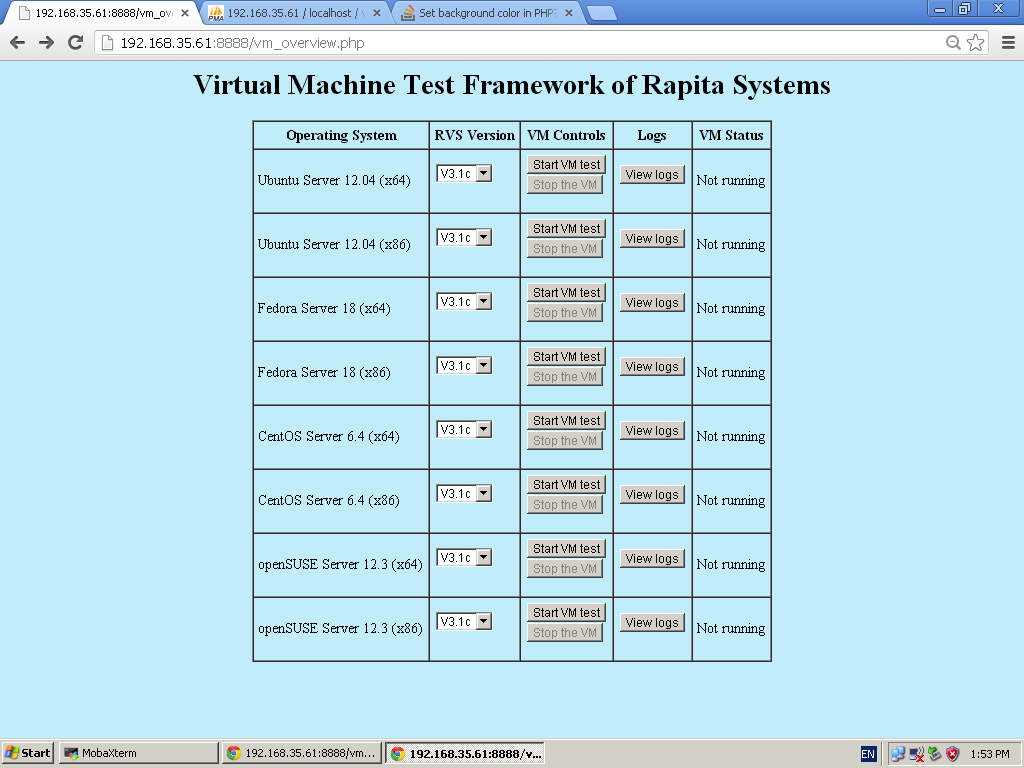
\includegraphics[width=1.4\textwidth, height=13.7cm]{framework.png}}%
  \caption{Front-end of Virtual Machine Test Framework of Rapita Systems}
  \label{fig:front}
\end{figure}

%\begin{figure}[h]
%\centering
%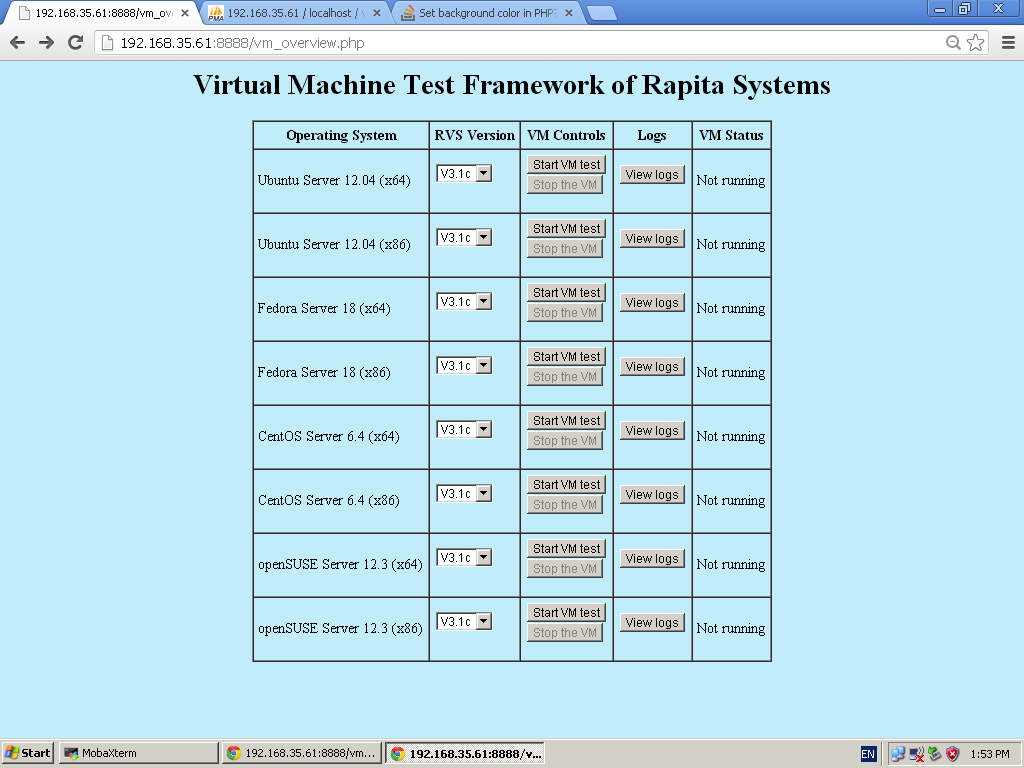
\includegraphics[width=14cm, height =12cm]{framework.png}
%\caption{Front-end of Virtual Machine Test Framework of Rapita Systems}
%\label{fig:front}
%\end{figure}

\noindent The front-end gets the available software versions from Software Server and the details of Guest VMs from the database to display on webpage. To initiate testing, the tester selects the RVS version with the desired operating system and clicks the ``Star VM Test'' button. Test is executed in the background and the tester can click the "Read Log" button to view the test results online, which can also be viewed later on from the log file.}\\

\noindent \textbf{\fontsize{14}{22}\selectfont {(6) Reverting Modifications after Test Completions:}} \\[0.2\baselineskip] 
\fontsize{11}{22}\selectfont {Once the test is completed, it is necessary to delete the modifications in order to avoid any interference in the future tests. A clean up script is placed for the purpose to uninstall the installed RVS software, delete the created folders, script files and safely shutdown the Guest VM.}\\

\noindent \textbf{\fontsize{14}{22}\selectfont {Working of the Testing System:}} \\[0.2\baselineskip] 
\indent \fontsize{11}{22}\selectfont {The step by step procedure of the system is explained in the Figure \ref{fig:process} with steps given below.}


\begin{figure}[h]
  \makebox[\textwidth][c]{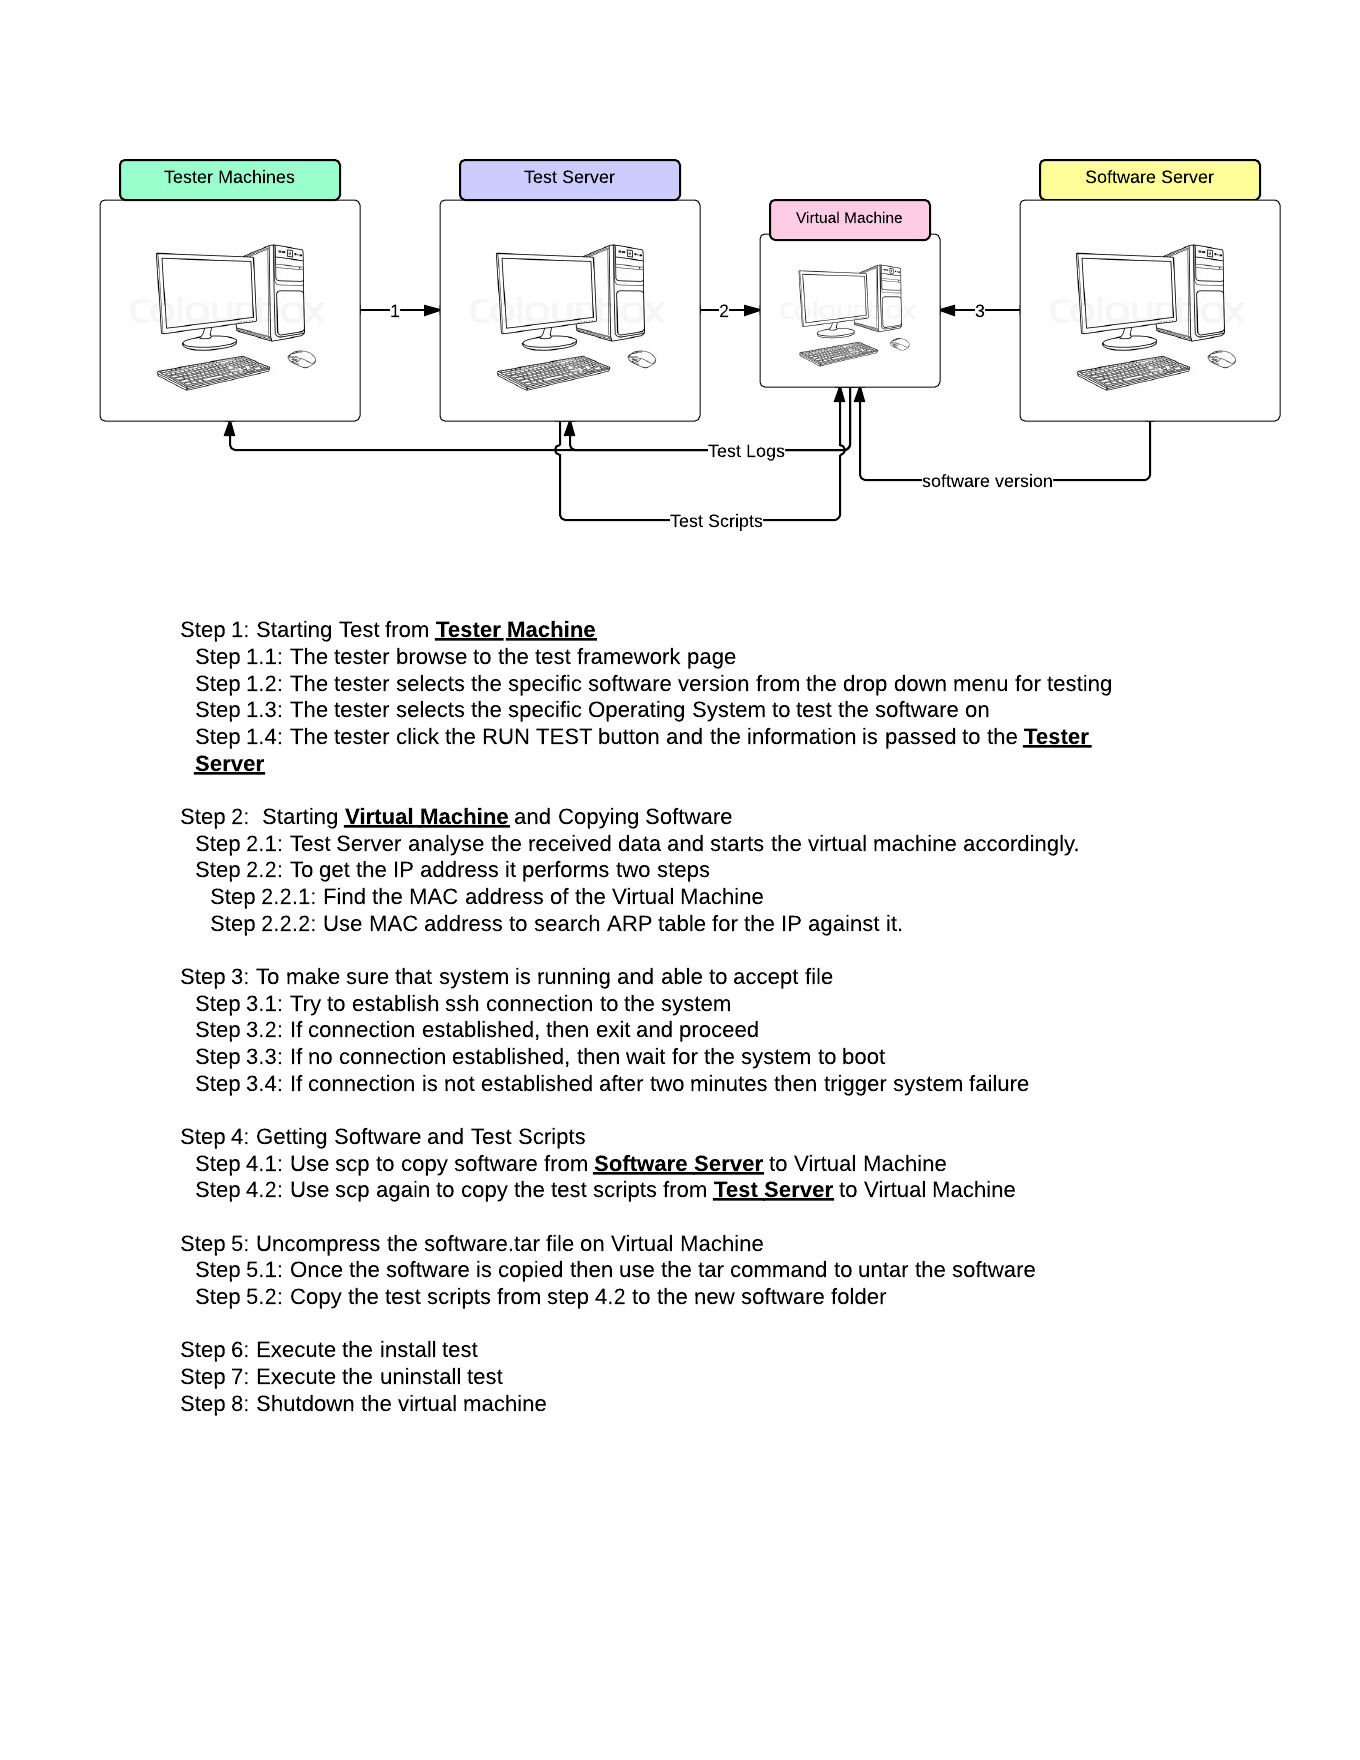
\includegraphics[width=1.2\textwidth, height=12cm]{rapitaSystems.png}}%
  \caption{Step by step process of the software testing}
  \label{fig:process}
\end{figure}


%\begin{figure}[h]
%\centering
%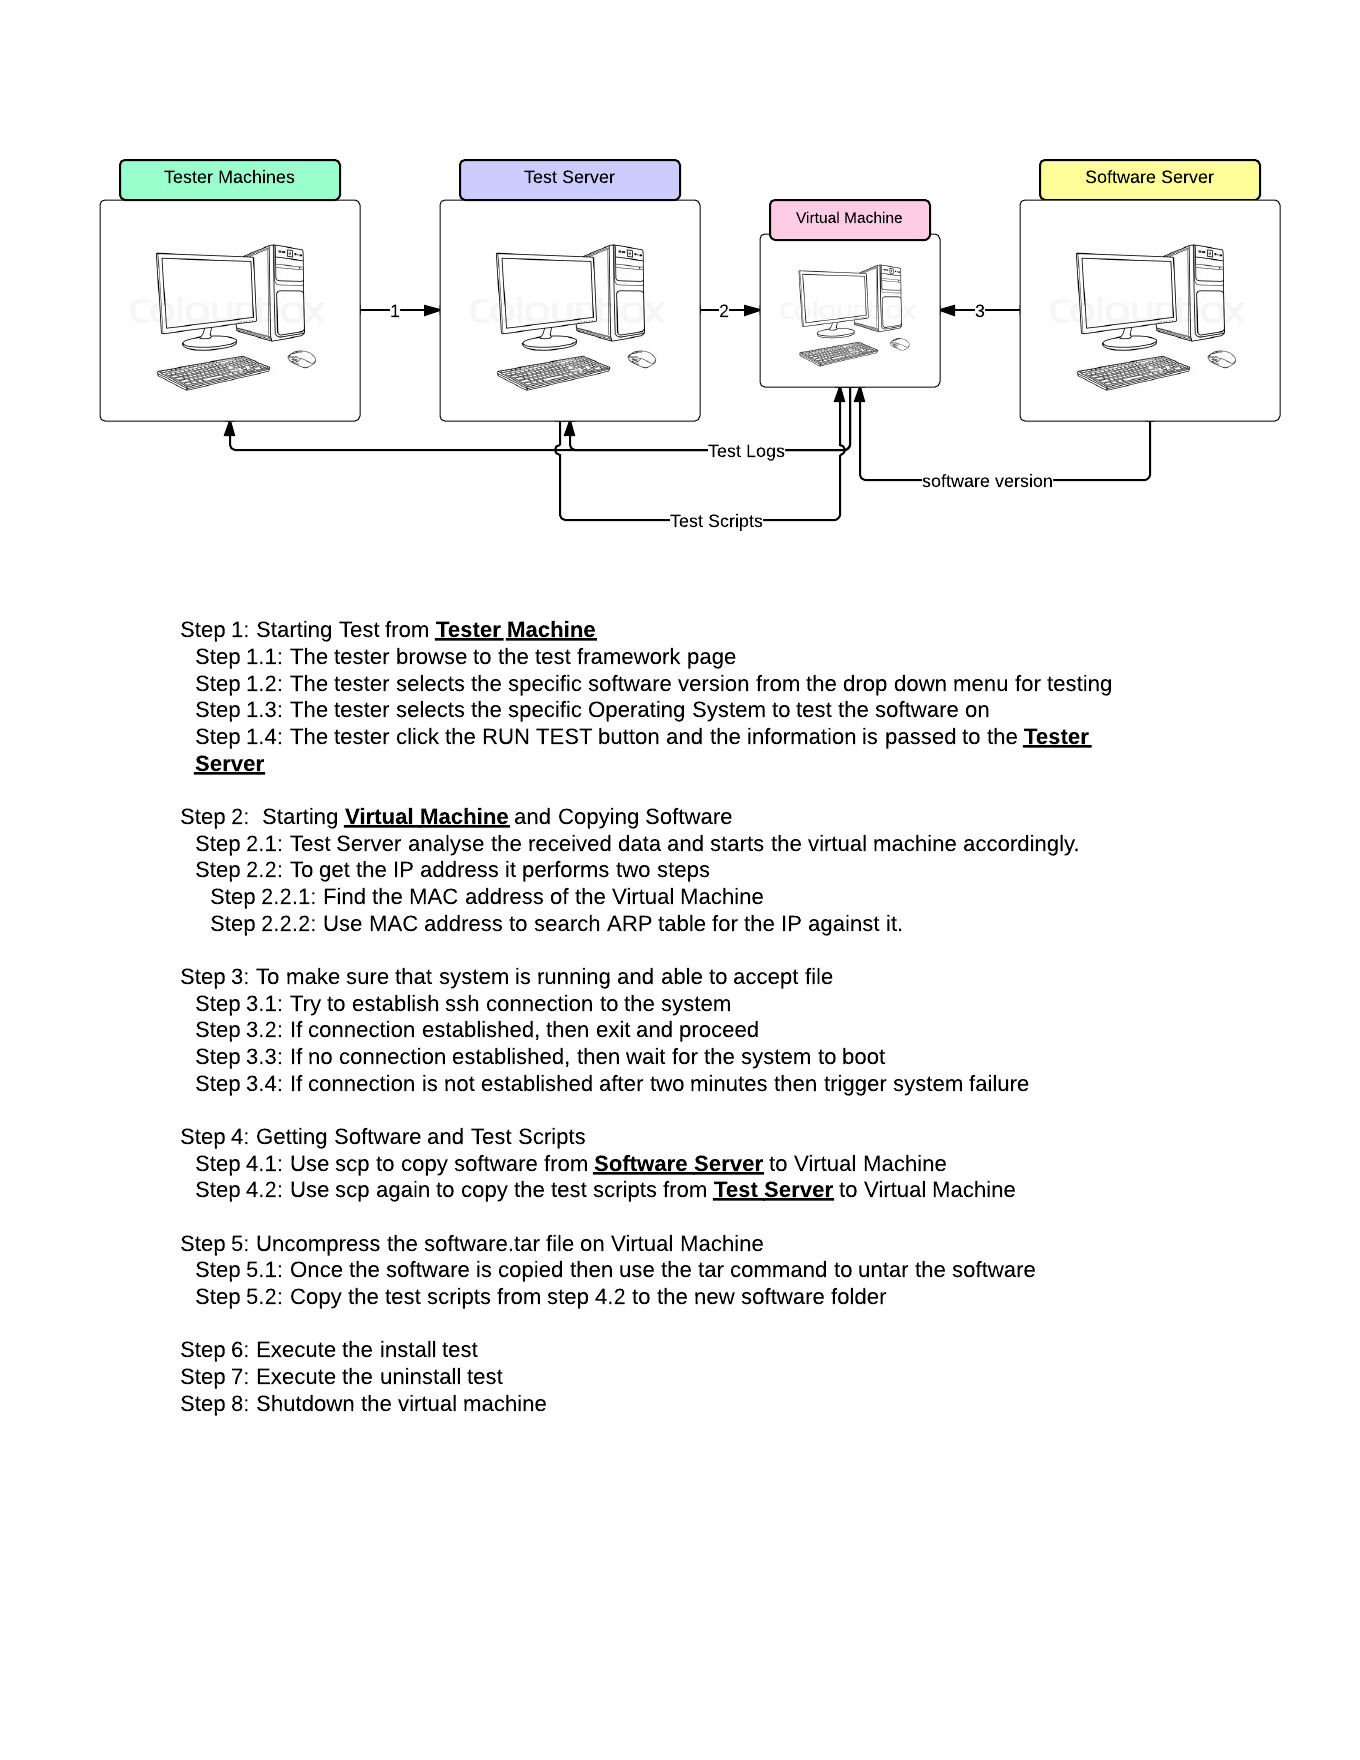
\includegraphics[width=11cm]{rapitaSystems.png}
%\caption{Step by step process of the software testing}
%\label{fig:process}
%\end{figure}

\noindent \textbf{\fontsize{14}{22}\selectfont {Future Work:}} \\[0.2\baselineskip] 
\indent {\fontsize{11}{22}\selectfont {
Some additional features, beyond the scope of current project were identified which may be explored in the future to make the system more efficient. \\
These features include:
\begin{enumerate}
\item Load balancing on test server to restrict specific number of VMs running at a time.
\item Automatic sending of the test log file as email to the tester after every test execution.
\item Creating more sophisticated test suites to execute after automated installation prior to uninstallation of RVS.
\item Adding more operating systems to the virtual box.
\item Designing more attractive front-end website.
\item Installing new operating system in the Virtualbox through a web page according to the requirements.
\end{enumerate}
}

\bigskip
\bigskip
\noindent \textbf{\fontsize{14}{22}\selectfont {Personal Note:}} \\[0.2\baselineskip] 
\fontsize{11}{22}\selectfont {My experience of internship at Rapita Systems was great. The company has a magnificent working environment and great minds contributing to very high quality work. I learnt a lot about test automation, instrumentation, data tracing regression testing and compatibility testing. 
%The project I completed is very satisfactory and highly appreciated by the whole team of Rapita Systems. 
This internship provided me the opportunity to have professional hands on experience which opened new horizons and broadened my knowledge gained at the academic institution.}\ \

\end{document}


